\documentclass[a4paper,12pt]{report}

\usepackage{alltt, fancyvrb, url}
\usepackage{graphicx}
\usepackage{subfigure}
\usepackage{wrapfig}
\usepackage{algorithmic}
\usepackage[utf8]{inputenc}
\usepackage{fontenc}
\usepackage{amsmath,stmaryrd,mathtools,algorithm}
\usepackage{amssymb}
\usepackage{float}
\usepackage{hyperref}
\usepackage{titlesec}
\newcommand{\sectionbreak}{\clearpage}
\newcommand{\subsectionbreak}{\clearpage}
\newcommand{\subsubsectionbreak}{\clearpage}

% Remove option to use English naming
\usepackage[italian]{cleveref}

% Questo commentalo se vuoi scrivere in inglese.
\usepackage[italian]{babel}

\title{Relazione per\\``DPG - Dope Party Game''}

\author{Davide Freddi\\Davide Picchiotti\\Miriana Ascenzo\\Riccardo Squarcialupi}
\date{\today}

\begin{document}

	\maketitle

	\tableofcontents

	\chapter{Analisi}
	\section{Requisiti}
	Il software DPG - Dope Party Game consiste in un gioco a turni, in cui l'obiettivo è far arrivare il proprio personaggio in fondo a un tabellone, costituito da uno o più percorsi formati da caselle.
	%
	Alla fine di ogni turno, vengono fatti fare dei minigiochi a ogni giocatore.

	\subsubsection{Requisiti funzionali}
	\begin{itemize}
		\item il software deve presentare un menu principale all'avvio, che permetta di avviare il gioco con diverse opzioni, quali numero di giocatori e numero di CPU
		\item il gioco viene giocato da più giocatori nello stesso computer, prendendo il controllo durante il proprio turno
		\item ai giocatori viene fatto tirare un dado, che determina quanti passi vengono fatti all'interno del tabellone
		\item esistono diversi tipi di celle, che possono causare diversi eventi quando un personaggio ci finisce sopra
		\item alla fine di ogni turno viene scelto casualmente un minigioco da far fare a tutti i giocatori, e in base alla posizione nella classifica dei punteggi vengono assegnati dadi migliori o peggiori
		\item ogni CPU ha una difficoltà, che determina i suoi punteggi nei minigiochi
		\item i minigiochi possibili sono:
		\begin{itemize}
			\item ballgame - bisogna far arrivare una palla in fondo a un percorso il prima possibile, e alcuni muri fanno tornare all'inizio se colpiti
			\item punchygame - bisogna colpire piu' sacchi possibili, mirando nella direzione giusta
			\item molegame - bisogna colpire più talpe possibili entro lo scadere del tempo
			\item jumpgame - bisogna arrivare più in alto possibile rimbalzando su delle piattaforme
		\end{itemize}
	\end{itemize}

	\section{Analisi e modello del dominio}

	Il programma partirà da un menu, che al momento opportuno avvierà il gioco.
	%
	All'avvio del gioco il menu notificherà il ciclo di gioco (GameCycle), che gestirà una serie di personaggi (Character).
	%
	I personaggi si muovono all'interno di una griglia (Grid) composta da caselle (Cell), e possono essere controllati o da un giocatore, o da una cpu (CPU), gestita del ciclo di gioco.
	%
	Alla fine del turno il gamecycle avvierà dei minigiochi (Minigame), che ritorneranno un certo punteggio intero.
	%
	Le difficlotà primarie potrebbero essere le seguenti:
	\begin{itemize}
		\item gestire le cpu in maniera intelligente, evitando di complicare eccessivamente il codice
		\item generare una griglia senza impostarne tutti i dettagli manualmente dal codice
		\item generare diverse configurazioni di griglie con un codice flessibile
		\item individuare una struttura di codice basilare e comune per i minigiochi
		\item gestire le collisioni e la fisica nei minigiochi che lo richiedono
	\end{itemize}

	\begin{figure}[!t]
		\centering{}
		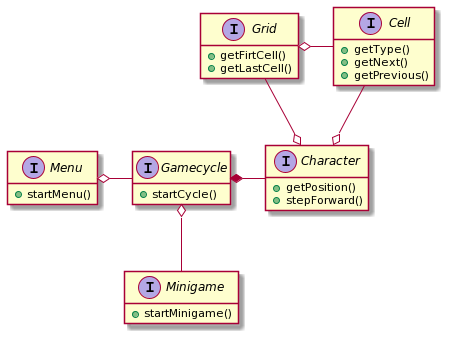
\includegraphics{images/domain.png}
		\caption{Schema UML dell'analisi del problema, con rappresentate le entità principali ed i rapporti fra loro}
		\label{img:analysis}
	\end{figure}

	\chapter{Design}

	\section{Architettura}

	L'architettura del software segue il pattern architetturale MVC.
	%
	Il menu è composto da una View (MenuView), e un Controller (MenuController) che ne cattura gli eventi e ne comanda le modifiche.
	%
	Quando il gioco viene avviato il Controller del menu avvia il ciclo di gioco (GameCycle).
	%
	Il ciclo di gioco avvia un nuovo thread in background che si occupa di gestire una serie di personaggi e le varie CPU, gestire la sequenza dei turni nel gioco, e aggiornare la View della griglia (Gridview) quando necessario.
	%
	Il Character rappresenta un personaggio in grado di tirare il proprio dado e spostarsi all'interno della griglia (Grid).
	%
	La CPU si occupa invece di fare le decisioni che spetterebbero normalmente al giocatore, come scegliere il percorso da fare in un bivio.
	%
	Il Character tiene traccia della propria posizione tramite un riferimento alla casella (Cell) su cui si trova.
	%
	La casella contiene delle coordinate e il riferimento alle caselle successive e precedenti nel tabellone.
	%
	La griglia gestisce le caselle, e permette di ottenere la prima e l'ultima casella del percorso, o una certa casella date delle coordinate.
	%
	Minigame si occupa di eseuire il minigioco, o ottenere un punteggio per una CPU in base alla sua difficoltà.
	%
	Ogni minigioco avrà a sua volta delle ulteriori interfacce di View, Controller e Model.

	\begin{figure}[!t]
		\centering{}
		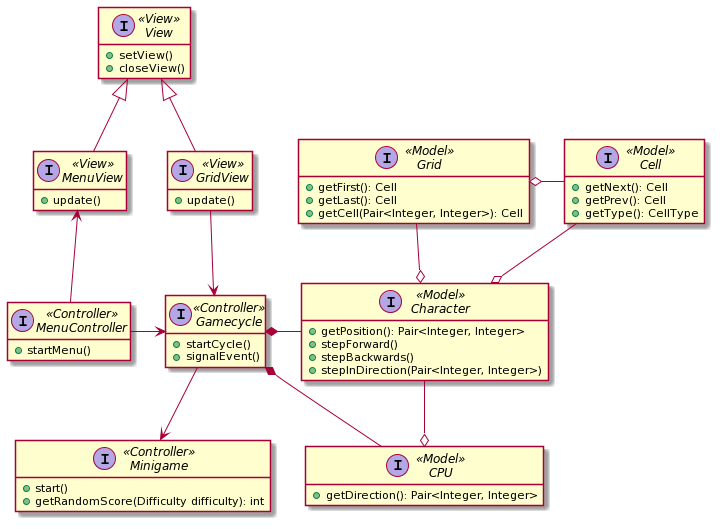
\includegraphics[width=\textwidth]{images/arch.png}
		\caption{Schema UML architetturale di DPG. View, GridView e MenuView sono interfacce di view, Gamecycle e Minigame sono interfacce di controller, mentre Grid, Cell e Character sono interfacce di modello.}
		\label{img:goodarch}
	\end{figure}
	%
	\section{Design Dettagliato}
	%
	\subsection{Design dettagliato Davide Freddi}
	\subsubsection{Player controller}
    \begin{figure}[h]
    \centering{}
    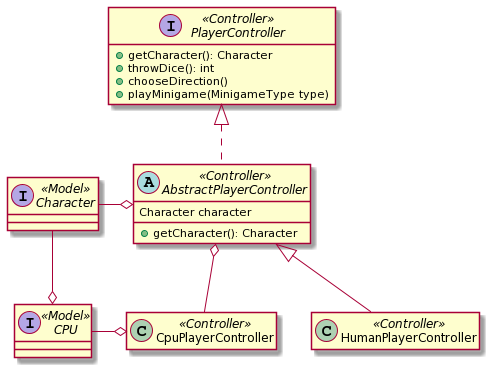
\includegraphics[width=\textwidth]{images/freddi/PlayerControllerImg.png}
    \caption{Uml del design di PlayerController.}
    \label{img:goodarch}
    \end{figure}

    Per gestire le operazioni che richiedono comportamenti diversi tra cpu e giocatori umani all'interno del ciclo di gioco, è stata creata l'interfaccia PlayerController con HumanPlayerController e CpuPlayerController come implementazioni.
    %
    Questo permette a un PlayerController, una volta istanziato, di essere usato indipendentemente da se si tratti di una cpu o un giocatore umano.
    %
    I PlayerController contengono al loro interno il Character da controllare, e CpuPlayerController in particolare contiene la CPU relativa al Character da controllare.

    \subsubsection{Turn manager}
    \begin{figure}[h]
    \centering{}
    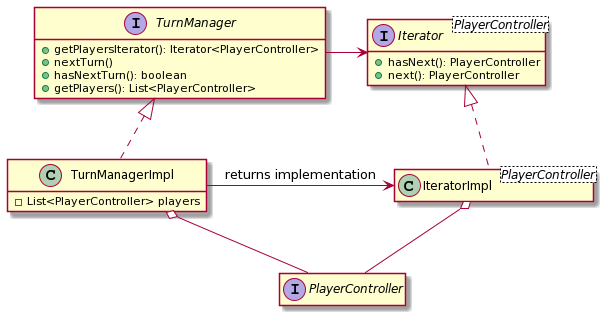
\includegraphics[width=\textwidth]{images/freddi/TurnManager.png}
    \caption{UML di TurnManager, gli elementi rappresentati fanno parte del controller.}
    \end{figure}
    TurnManager gestisce i PlayerController durante il corso della partita, decidendone l'ordine dei turni e svolgendo le operazioni da svolgere alla fine di ogni turno (quali l'esecuzione dei minigiochi e l'assegnazione dei dadi in base ai punteggi ottenuti).
    %
    TurnManager utilizza il pattern \textbf{iterator}, restituendo un Iterator di PlayerController a ogni turno che scorre i player nell'ordine in cui devono svolgere il loro turno.
    %
    In questa istanza di iterator TurnManager è l'aggregate, Iterator è l'iterator, TurnManagerImpl è il concrete aggregate, IteratorImpl è il concrete iterator e GamecycleImpl è il client che sfrutta l'iterator e l'aggregate.

    \subsubsection{PlayerFactory}
    \begin{figure}[h]
    \centering{}
    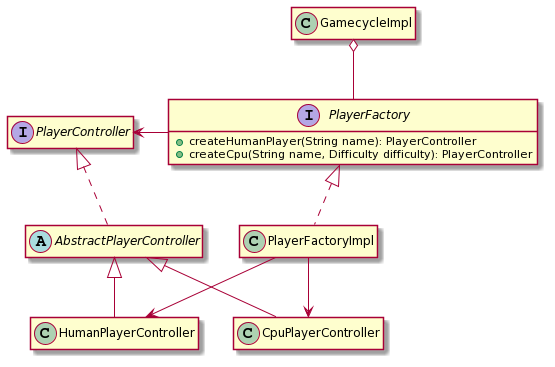
\includegraphics[width=\textwidth]{images/freddi/PlayerFactory.png}
    \caption{UML di PlayerFactory, gli elementi rappresentati fanno parte del controller.}
    \end{figure}

    Per isolare la parte di inizializzazione di un PlayerController (che comprende tra le altre cose la creazione di un Character), dall'utilizzo effettivo di quest'ultimo, è stata creata una PlayerFatory.
    %
    PlayerFactory utilizza \textbf{factory method} come pattern, e in questa istanza del pattern PlayerFactory è il creator, PlayerFactoryImpl è il concrete creator, PlayerController è il product e HumanPlayerController e CpuPlayercontroller sono i concrete product.

    \subsubsection{Turn manager builder}
    \begin{figure}[h]
    \centering{}
    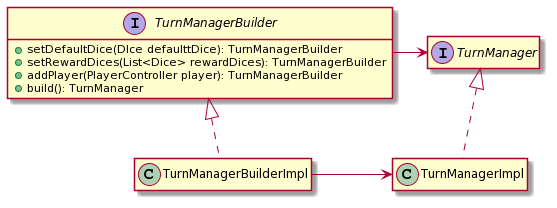
\includegraphics[width=\textwidth]{images/freddi/TurnManagerBuilder.png}
    \caption{UML di TurnManagerBuilder, gli elementi rappresentati fanno parte del controller.}
    \end{figure}

    TurnManagerBuilder serve per generare un TurnManager in maniera agevole tramite il pattern \textbf{builder}.
    %
    In questa istanza di builder TurnManagerBuilder è il builder, TurnManager è il Product e GamecycleImpl è il director che utilizza il builder per creare il product.

    \subsubsection{Gamecycle e gamecycle builder}
    \begin{figure}[h]
    \centering{}
    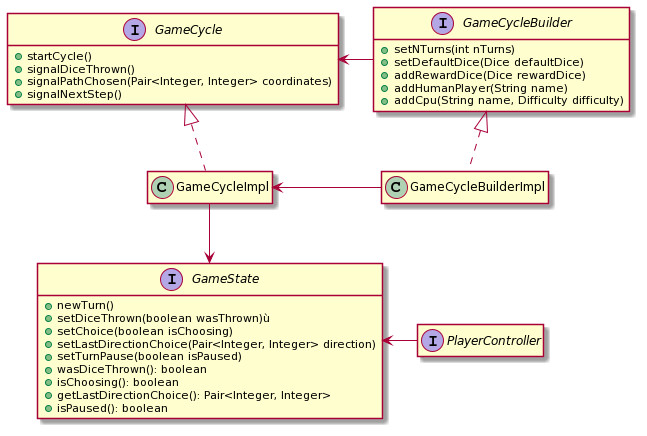
\includegraphics[width=\textwidth]{images/freddi/GameCycle.png}
    \caption{UML di Gamecycle, gli elementi rappresentati fanno parte del controller.}
    \end{figure}

    GamecycleBuilder viene utilizzato da MenuController, e seguendo il pattern \textbf{builder} genera il Gamecycle.
    %
    Questo da la possibilità all'utilizzatore del builder di creare un gamecycle che esegua una partita con regole diverse, in base alle esigenze.
    %
    Il gamecycle crea un thread che esegue le operazioni in background, aggiornando la view quando necessario.
    %
    GameState esiste per tenere traccia dei vari stati del gioco, nel GameCycle viene creata una sola istanza di GameState e sia il GameCycle sia i PlayerController possono accedervi per leggere o modificare lo stato del gioco.
    %
    L'istanza di GameState viene inoltre usata per la sincronizzazione del thread del gamecycle con gli altri thread.

    \subsubsection{Ball minigame}
    \begin{figure}[h]
    \centering{}
    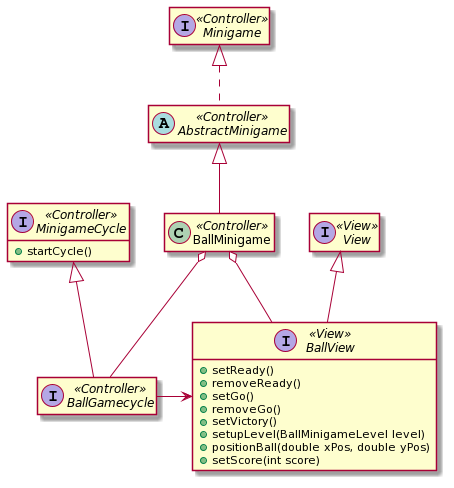
\includegraphics[width=\textwidth]{images/freddi/BallMinigame.png}
    \caption{UML semplificato di BallMinigame.}
    \end{figure}

    Il minigioco BallMinigame si compone di un ciclo di gioco, che attua delle modifiche su una view tramite la sua interfaccia.
    %
    Vengono estese le classi astratte dei minigiochi.

    \subsubsection{Ball observer}
    \begin{figure}[h]
    \centering{}
    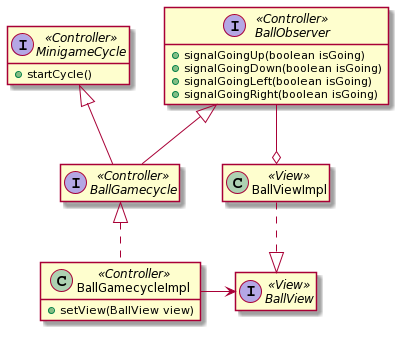
\includegraphics[width=\textwidth]{images/freddi/BallObserver.png}
    \caption{UML di BallObserver.}
    \end{figure}

    Viene usato il pattern \textbf{observer} per catturare gli input della view, ricevendo le informazioni necessarie per aggiornare il proprio stato.
    %
    In questa istanza di observer BallView è il subject, BallViewImpl è il concrete subject, BallObserver è l'observer e BallGamecycleImpl è il concrete observer.

    \subsubsection{Nodes factory}
    \begin{figure}[h]
    \centering{}
    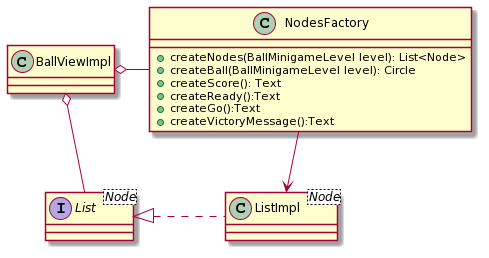
\includegraphics[width=\textwidth]{images/freddi/NodesFactory.png}
    \caption{UML di BallObserver, tutti gli elementi fanno parte della view.}
    \end{figure}

    Questa classe serve per creare i nodi necessari alla view.
    %
    NodesFactory segue il pattern \textbf{simple factory}, in quanto restituisce tramite il metodo createNodes un'implementazione di List[Node] che cambia in base al BallMinigameLevel passato come parametro.
    %
    Questo permette di creare una serie di view per diversi livelli in maniera agevole.
    %
    Dato che la dimensione della view varia in base alla dimensione dello schermo, viene passata l'implementazione di una Function che serve per mappare le coordinate dei nodi in modo da adattarli alla dimansione della view.
    %
    Si fa quindi uso del pattern \textbf{strategy}, in cui NodesFactory è il context e Function è la strategy, che viene implementata da BallViewImpl quando istanzia NodesFactory.

    \subsubsection{Ball minigame model}
    \begin{figure}[h]
    \centering{}
    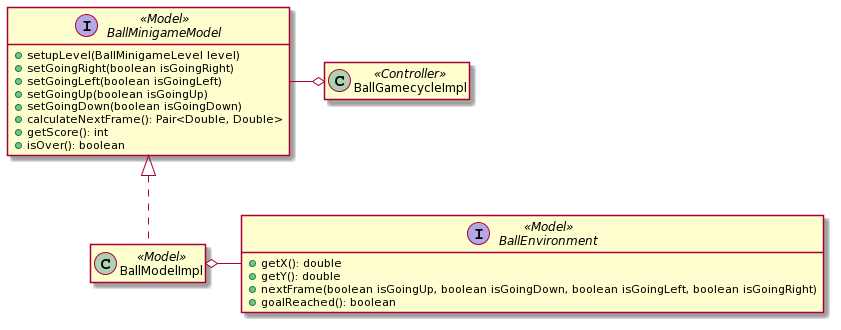
\includegraphics[width=\textwidth]{images/freddi/BallMinigameModel.png}
    \caption{UML di BallMinigameModel}
    \end{figure}

    BallMinigameModel è l'unica interfaccia di modello a cui il Gamecycle fa riferimento.
    %
    Permette di selezionare il livello da giocare, settando così un certo comportamento per la pallina.
    %
    Permette inoltre di ottenere informazioni sulla partita ad ogni frame, in base all'input del giocatore che viene notificato al modello tramite gli appositi metodi.
    %
    Gestice inoltre il punteggio, che cala mano a mano col passare del tempo.
    %
    Il modello richiede come parametro un valore di fps attesi, ovvero il numero di volte che si aspette di essere aggiornato ogni secondo.
    %
    Questo valore influenza il tempo calcolato tra un frame e l'altro per il movimento della palla nel livello.

    \subsubsection{Ball environment factory}
    \begin{figure}[h]
    \centering{}
    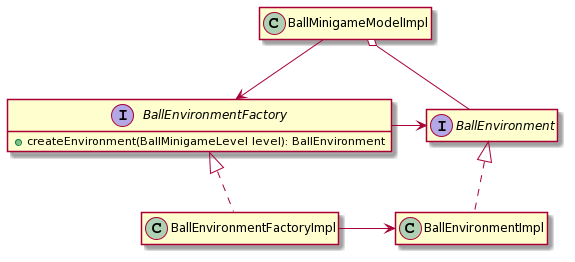
\includegraphics[width=\textwidth]{images/freddi/BallEnvironmentFactory.png}
    \caption{UML di BallEnvironmentFactory, tutti gli elementi fanno parte del model}
    \end{figure}

    Sfrutta il pattern \textbf{factory method} per generare un'istanza di BallEnvironment in base al livello passato al metodo createEnvironment.
    %
    Questo permette la creazione di diversi livelli in maniera agevole, cambiando semplicemente l'implementazone di ballEnvirmenr al variare dell'enum.
    %
    In questa istanza di factory method, BallEnvironmentFactory è il creator, BallEnvironmentFactoryImpl è il concrete creator, BallEnvironment è il prouct e BallEnvironmentImpl è il concrete product.

    \subsubsection{Ball environment}
    \begin{figure}[h]
    \centering{}
    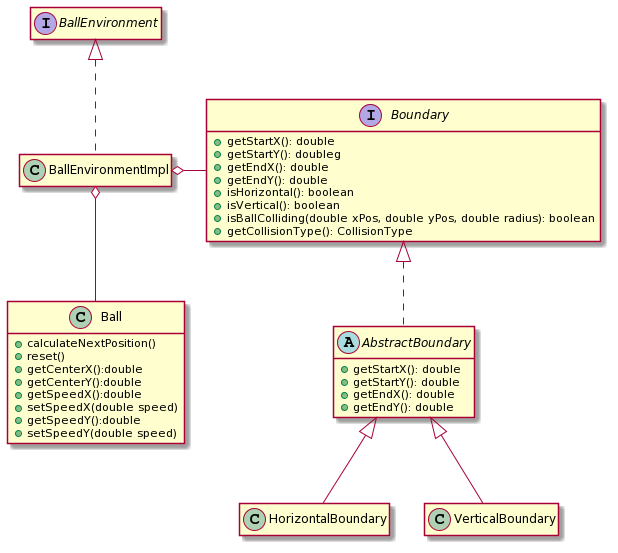
\includegraphics[width=\textwidth]{images/freddi/BallEnvironment.png}
    \caption{UML di BallEnvironment, tutti gli elementi fanno parte del model}
    \end{figure}

    BallEnvironment è l'ambiente in cui la palla si muove e collide contro i muri.
    %
    A ogni frame viene ricalcolata la posizione della palla, si controlla se collide o meno con un muro e si gestisce la collisione nel caso.
    %
    Boundary rappresenta un muro, identificato con punti di inizio, fine e tipo di collisione.
    %
    Nonostante Boundary sia stato implementato solo con HorizontalBoundary e VerticalBoundary, l'interfaccia Boundary può essere implementata in diversi modi, anche con boundary con angolazioni diverse, che complicano il calcolo della collisione con la palla.
    %
    HorizontalBoundary e VertivalBoundary erano tuttavia sufficienti per ball minigame, in quanto i muri sono o verticali o orizzontali.

	\subsection{Design dettagliato Davide Picchiotti}
	\subsubsection{Modellazione dei giocatori}
	In questa sezione si tratterà il design dei giocatori all'interno del modello.\newline
	\newline
	Ogni giocatore (umano e non) viene rappresentato tramite l'interfaccia Character.
	Questo espone metodi per controllare tutti gli aspetti relativi a un dato giocatore durante la partita:
	\begin{itemize}
		\item movimento step-by-step nella griglia
	    \item lancio di dado
	    \item salvataggio di valori importanti durante la partita (turno, posizione, punteggio dei minigiochi ecc.)
	\end{itemize}
	%
	L'avanzamento del giocatore con gli appositi metodi avviene step-by-step, ovvero si muoverà di una
	casella per ogni chiamata; è stata presa questa direzione di design per fare in modo che durante
	uno stesso lancio di dado, tra una casella e l'altra, si potessero scatenare eventi sul giocatore
	dovuti dal tipo di casella attraversata.\newline
	%
    \begin{figure}[h]
        \centering{}
        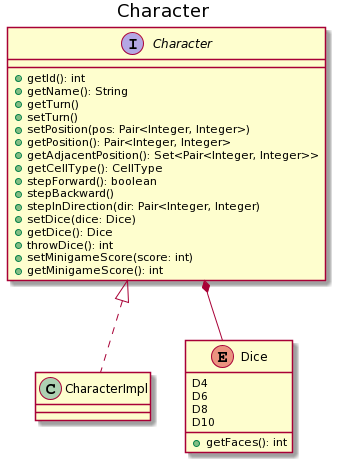
\includegraphics{images/picchiotti/character.png}
        \caption{Schema UML dell'interfaccia Character}
        \label{img:character}
    \end{figure}
	%
	Per fare in modo che nella partita siano presenti giocatori non umani (CPU) è necessario servirsi
	dell'interfaccia Cpu.\newline
	Le sue implementazioni dovranno contenere un Character in modo da poter "prendere le decisioni" in vece del giocatore, come la direzione da prendere a un bivio.\newline
	Inoltre ogni Cpu avrà assegnata una difficoltà (enum Difficulty) che al momento stabilisce unicamente il punteggio che otterrà nei minigiochi.\newline
	In questo modo è possibile creare nuovi tipi di Cpu con diversi comportamenti in maniera disaccoppiata.
	%
    \begin{figure}[!t]
        \centering{}
        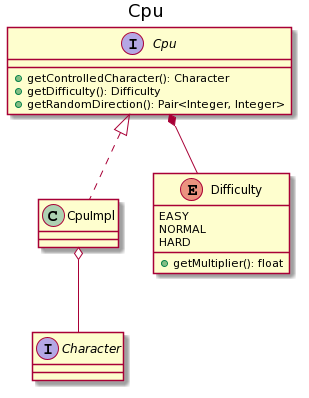
\includegraphics{images/picchiotti/cpu.png}
        \caption{Schema UML dell'interfaccia Cpu}
        \label{img:cpu}
    \end{figure}

	\subsubsection{Struttura base dei minigiochi}
	In questa sezione si tratterà delle classi e interfaccie che stanno alla base di tutti i minigiochi del progetto.\newline
	\newline
	I minigiochi sono stati trattati come piccoli progetti a sé stanti da integrare poi nel gioco completo, con il semplice requisito che ognuno di essi ritorni un punteggio intero.\newline
	%
	Le classi e le interfaccie presentate sono state pensate con lo scopo di avere un buona struttura MVC per ogni minigioco e allo stesso tempo aver un entry-point definito per l'avvio e il settaggio di qualunque minigioco. L'unica parte architetturale che non viene definita da questa struttura è il Model di ognuno, poiché considerato troppo specifico in base al tipo di minigioco che si intende realizzare.\newline
	%
    \begin{figure}[!t]
        \centering{}
        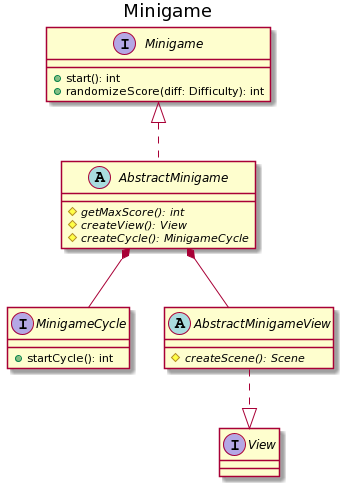
\includegraphics{images/picchiotti/minigame.png}
        \caption{Schema UML della struttura generale dei minigiochi}
        \label{img:minigame}
    \end{figure}
	%
	Per far sì che la routine di avvio e settaggio del minigioco fosse uguale per ognuno si è adottata la strategia delle classi astratte con Template Method.
	Nello specifico AbstractMinigameView ha il metodo template createScene() per la creazione della Scene di JavaFX e AbstractMinigame ha i metodi template getMaxScore (per il calcolo del punteggio), createGameCycle() (per la creazione del ciclo di gioco) e createView() (per la creazione della View).\newline
	Inoltre l'interfaccia Minigame ha l'unico metodo start() che fornisce un entry-point univoco per qualunque minigioco implementato in maniera corretta.\newline
	\newline
	Il punto debole di questa soluzione è che le classi astratte proposte andranno modificate o sostitutite se si sceglie di utilizzare un componente grafico diverso da JavaFX. Mettendo sulla bilancia questo aspetto negativo con quello positivo di poter "generalizzare" il comportamento del minigioco alle fondamenta, è stato considerata comunque una soluzione valida per la quantità esigua di modifiche che richiederebbe la sostituzione del componente grafico.

	\subsubsection{Punchy Minigame}
	In questa sezione verrà trattato nel dettaglio il design del minigioco Punchy.\newline
	\newline
	Per il design di questo minigioco ci si è per lo più limitati a implementare le opportune interfacce e a estendere le classi astratte.
    Sono state create interfacce aggiuntive per la gestione della View (PunchyminigameView) e del Model (World).
    \begin{figure}[!t]
        \centering{}
        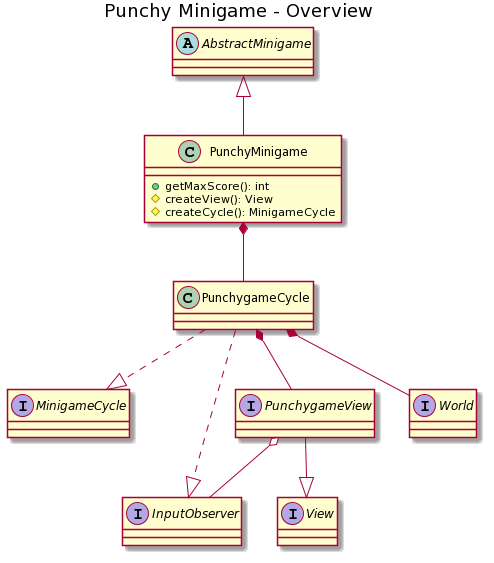
\includegraphics{images/picchiotti/punchyoverview.png}
        \caption{Schema UML generale del minigioco Punchy}
        \label{img:punchyoverview}
    \end{figure}

	In generale, l'interfaccia PunchygameView permette di gestire tutti gli aspetti della View che rispecchiano il Model del gioco, ma la classe che la implementa necessita anche l'estensione di AbstractMinigameView per poter settare e chiudere la View stessa.
    L'interfaccia consente comunque di scorporare la View e di cambiare in maniera agevole il componente grafico.\newline
    \begin{figure}[h]
        \centering{}
        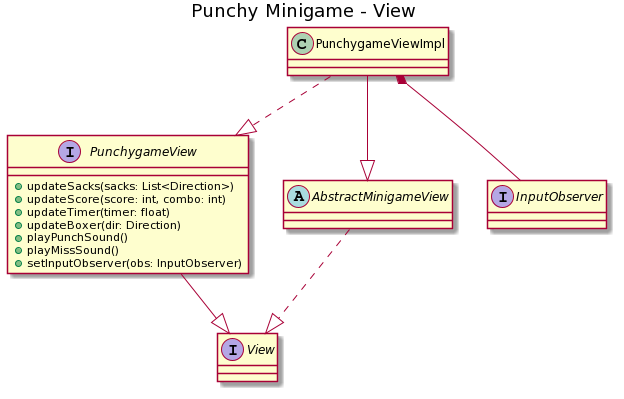
\includegraphics[width=150mm]{images/picchiotti/punchyview.png}
        \caption{Schema UML del componente View}
        \label{img:punchyview}
    \end{figure}

	Inoltre è stato utilizzato il pattern Observer per la gestione degli input dell'utente: la View (PunchygameView) è il componente osservato, mentre l'osservatore sarà nel Controller (PunchygameCycle) e otterrà gli input tramite InputObserver.\newline
	Gli input da propagare verso il Controller sono modellati con l'interfaccia Input, che con pattern Strategy ci permette di cambiare a seconda delle esigenze gli input da passare a InputObserver.
    Essendo necessari solo due comandi per rappresentare il pugno a destra e a sinistra (molto simili tra loro) si è optato per una classe astratta che implementa Input e fa uso del pattern Template Method per farsi fornire dai suoi sottotipi la Direction del pugno.
	Il metodo template in questione è getPunchDirection() in AbstractPunch.
    \begin{figure}[h]
        \centering{}
        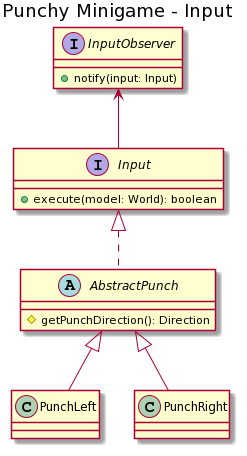
\includegraphics{images/picchiotti/punchyinput.png}
        \caption{Schema UML dei componenti di gestione di input}
        \label{img:punchyinput}
    \end{figure}

	%
	La parte di Model è molto semplice, in quanto presenta la classe World come unico entry-point del model, la cui implementazione userà al suo interno i vari componenti Boxer, Timer, Score. La componente dei sacchi da boxe del gioco non ha necessitato di una classe specializzata, poiché modellabile con una semplice lista all'interno di WorldImpl.\newline
    \begin{figure}[h]
        \centering{}
        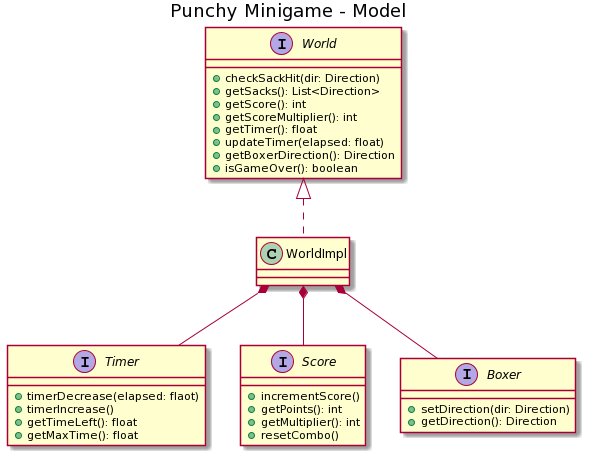
\includegraphics[width=150mm]{images/picchiotti/punchymodel.png}
        \caption{Schema UML del componente Model}
        \label{img:punchymodel}
    \end{figure}
	%
	La parte di Controller è costituita dal ciclo di gioco, ci si limita quindi a implementare l'interfaccia MinigameCycle.
    Naturalmente è necessario avere un InputObserver all'interno del Controller e si è optato per l'implentazione di esso direttamente nella classe PunchygameCycleImpl.
    \begin{figure}[!t]
        \centering{}
        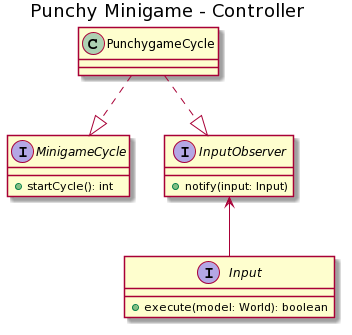
\includegraphics{images/picchiotti/punchycontroller.png}
        \caption{Schema UML del componente Controller}
        \label{img:punchycontroller}
    \end{figure}
	%

	\subsubsection{Jump Minigame}
	In questa sezione verrà trattato nel dettaglio il design del minigioco Jump.\newline
	\newline
	Per il design di questo minigioco ci si è per lo più limitati a implementare le opportune interfacce e a estendere le classi astratte. Sono state create interfacce aggiuntive per la gestione della View (JumpminigameView) e del Model (World).
    \begin{figure}[!t]
        \centering{}
        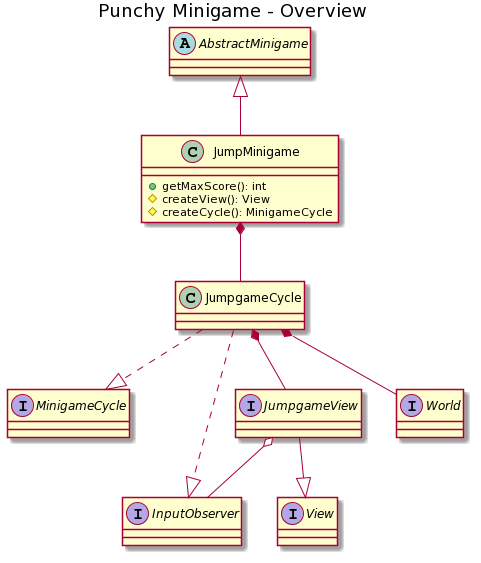
\includegraphics[width=140mm]{images/picchiotti/jumpoverview.png}
        \caption{Schema UML generale del minigioco Jump}
        \label{img:jumpoverview}
    \end{figure}

	In generale, l'interfaccia JumpgameView permette di gestire tutti gli aspetti della View che rispecchiano il Model del gioco, ma la classe che la implementa necessita anche l'estensione di AbstractMinigameView per poter settare e chiudere la View stessa.
    L'interfaccia consente comunque di scorporare la View e di cambiare in maniera agevole il componente grafico.\newline
    \begin{figure}[h]
        \centering{}
        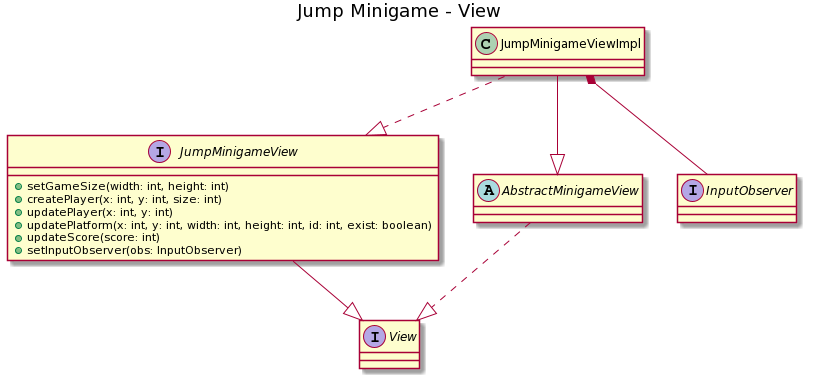
\includegraphics[width=150mm]{images/picchiotti/jumpview.png}
        \caption{Schema UML del componente View}
        \label{img:jumpview}
    \end{figure}

	Inoltre è stato utilizzato il pattern Observer per la gestione degli input dell'utente: la View (JumpminigameView) è il componente osservato, mentre l'osservatore sarà nel Controller (JumpgameCycle) e otterrà gli input tramite InputObserver.\newline
	Gli input da propagare verso il Controller sono modellati con l'interfaccia Input, che con pattern Strategy ci permette di cambiare a seconda delle esigenze gli input da passare a InputObserver.
	Nel caso di questo minigioco abbiamo tre comandi, ognuno dei quali modifica la velocità orizzontale del giocatore;
    per questo motivo è stata usata una classe astratta che utilizza il pattern Template Method per definire la velocità orizzantale da impostare al giocatore in ogni comando.
    \begin{figure}[h]
        \centering{}
        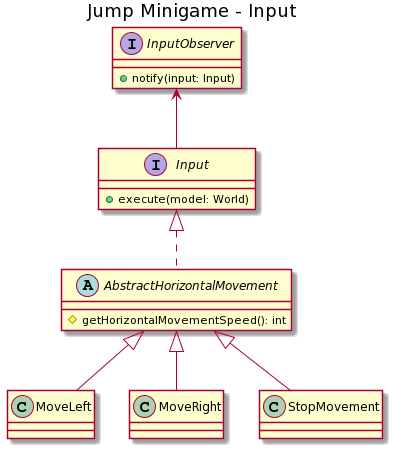
\includegraphics{images/picchiotti/jumpinput.png}
        \caption{Schema UML dei componenti di gestione dell'input}
        \label{img:jumpinput}
    \end{figure}
	%
	La parte di Model è molto semplice, in quanto presenta la classe World come unico entry-point del model, la cui implementazione userà al suo interno i vari componenti Player, Platform, PlatformSpawner.\newline
	Come si può vedere dai diagrammi, sia Player che Platform sono sottoclassi di AbstractGameObject, implementazione di base di GameObject.
    In questo modo è stata definita un'interfaccia generale per gli oggetti di gioco in grado di muoversi.\newline
    \begin{figure}[h]
        \centering{}
        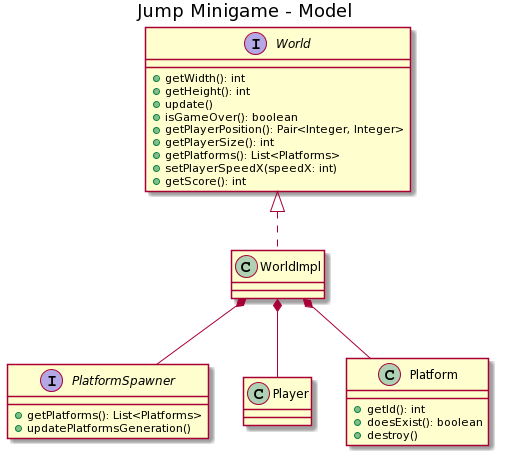
\includegraphics[width=150mm]{images/picchiotti/jumpmodel.png}
        \caption{Schema UML del componente Model}
        \label{img:jumpmodel}
    \end{figure}
	%
	La parte di Controller è costituita dal ciclo di gioco, ci si limita quindi a implementare l'interfaccia MinigameCycle.
    Naturalmente è necessario avere un InputObserver all'interno del Controller e si è optato per l'implentazione di esso direttamente nella classe JumpgameCycleImpl.
    \begin{figure}[!t]
        \centering{}
        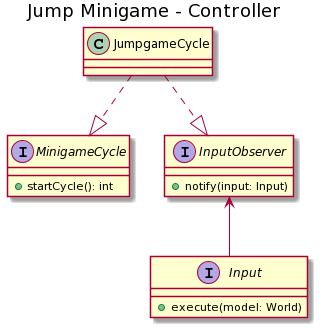
\includegraphics[width=150mm]{images/picchiotti/jumpcontroller.png}
        \caption{Schema UML del componente Controller}
        \label{img:jumpcontroller}
    \end{figure}
	%

	\subsection{Design dettagliato Miriana Ascenzo}
    \subsubsection {modello Grid}
	In modello, una classe GridInitializer si occupa della creazione di una Grid, ovvero un Tabellone di Gioco, partendo da un GridType.
	%
	GridInitializer cerca, in base al tipo di Griglia passatogli, un file json corrispondente: tale file viene letto tramite l'uso della libreria Jackson.
	%
	La classe è stata sviluppata quindi in modo tale da rendere automatica la creazione di una grid diverse in base al json, seguendo sempre lo stesso procedimento.
	%
	I dati vengono letti raccolti dal json Cella per Cella, tramite la classe CellParser.
	%
	Vengono quindi create diverse Cell, che compongono una Grid.
    %
    Abbiamo un Pattern Builder, per cui abbiamo un builder GridInitializer che crea i il product Grid.

	\begin{figure}[h]
		\centering{}
		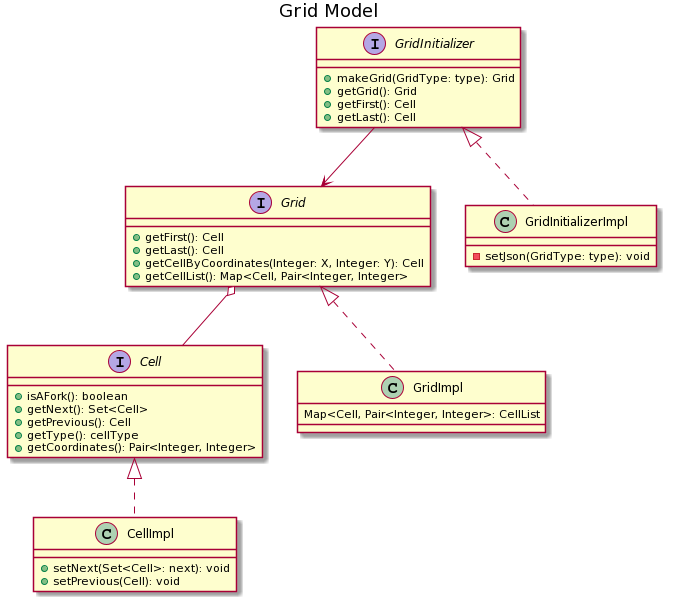
\includegraphics[width=150mm]{images/ascenzo/grid_model.png}
		\caption{Schema UML della generazione di una Grid e della sua struttura.}
		\label{img:gridmodel}
	\end{figure}

    \subsubsection {controller Grid}
	In controller, abbiamo una classe GridGenerator: tramite il suo unico metodo generate(), vengono creati prima una Grid, e poi una GridView basata su tale Grid.
	%
	Una Grid viene creata a partire dagli elementi che gli vengono forniti: GridGenerator prende per costruttore una GridType (enum di possibili griglie) e tramite essa cerca nelle resources un file Json corrispondente.
	%
	GridGenerator riceve inoltre un GameCycle: questo verrà passato a GridView affinchè la view generi il suo GridObserver.
    %
    GridGenerator è colui che usa il builder GridInitializer per creare i Product View e GridView.

	\begin{figure}[h]
	\centering{}
	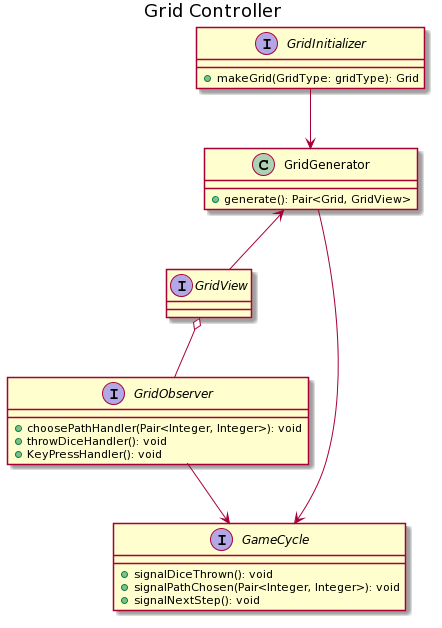
\includegraphics[width=130mm]{images/ascenzo/grid_controller.png}
	\caption{Schema UML del controller di Grid e di come interagisce con GameCycle}
	\label{img:gridcontroller}
	\end{figure}

    \subsubsection {Grid View}
	La View della Griglia estende da View, e viene in seguito implementata affinchè generi i nodi necessari.
	%
	La generazione di alcuni nodi ripetuti viene gestita in una classe ViewNodesFactory: essa genera le Celle in base alla posizione, le linee che collegano tali Celle, e i player.
	%
	La View può essere sostituita in blocco grazie al modello MVC: essa non riceve mai elementi di modello, solo riferimenti.

	\begin{figure}[h]
		\centering{}
		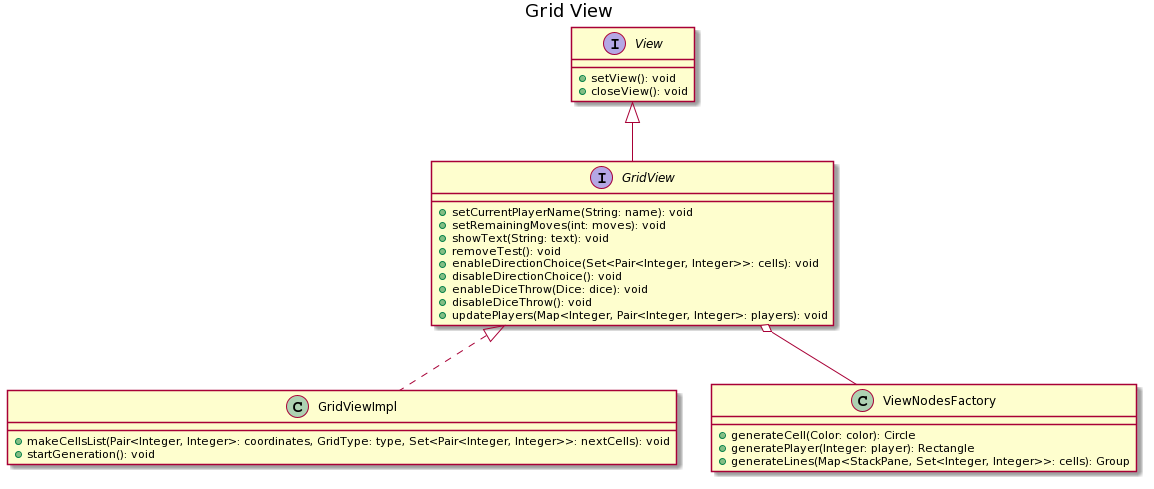
\includegraphics[width=150mm]{images/ascenzo/grid_view.png}
		\caption{Schema UML della View della Grid}
		\label{img:gridview}
	\end{figure}

    \subsubsection {Grid Observer}
	Gli elementi di GridView che ricevono input dall’esterno, ad esempio i bottoni, hanno il ruolo di informare il gameCycle di quale azione è stata intrapresa da chi sta usando il software.
	%
	Per questo viene generato GridObserver, una classe di pattern Observer.
	%
	La classe GridObserver ha per Observable GridViewImpl: Se un determinato bottone viene premuto, o una determinata key sulla tastiera viene premuta, viene inviato un segnale al GameCycle.

	\begin{figure}[h]
	\centering{}
	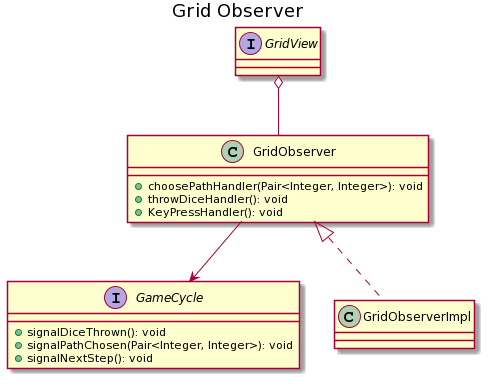
\includegraphics[width=\textwidth]{images/ascenzo/grid_observer.png}
	\caption{Schema UML dell'interazione fra GridView e GameCycle. Segue il pattern Observer.}
	\label{img:gridobserver}
	\end{figure}

    \subsubsection {Grid Proxy}
	I nodi di GridViewImpl vengono aggiornati in runtime ogni volta che gli elementi all’interno del software, quali players, dices, scritte da rappresentare, vengono modificati dal controller (ovvero il gameCycle).
	%
	Per aggiornare i nodi correttamente in runtime, esiste una classe GridViewPlat: quest'ultima implementa GridView, e riceve da GridGenerator una GridViewImpl.
	%
	GridViewPlat chiama i metodi di GridViewImpl nel thread dell’applicazione JavaFX.
	%
	Questo avviene tramite l’uso di Platform.runLater.
	%
	Quello che succede in GridGenerator è quindi: una GridViewImpl viene creata a partire da una Grid, e in seguito, a partire da GridViewImpl, viene creata una GridViewPlat, responsabile dell’aggiornamento della View nel thread dell’applicazione JavaFX.
	%
	Abbiamo un pattern Proxy, per cui gameCycle accede a GridViewPlat (proxy), il quale contiene GridViewImpl (real target), per aggiornare la View.

	\begin{figure}[h]
	\centering{}
	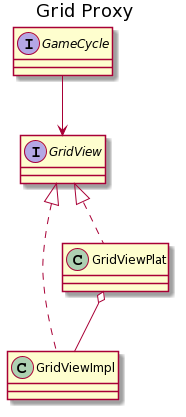
\includegraphics[width=80mm]{images/ascenzo/grid_proxy.png}
	\caption{Schema UML di come GameCycle accede a GridViewImpl. Segue il pattern Proxy.}
	\label{img:gridmediator}
	\end{figure}

	\subsection{Design dettagliato Riccardo Squarcialupi}
	Design dettagliato Riccardo Squarcialupi

	\chapter{Sviluppo}
	\section{Testing automatizzato}

	\subsection{Davide Freddi}
	I test sono stati eseguiti con junit5, Mockito, e testFx per le view.
    %
    Sono stati eseguiti dei test automatici sulle classi principali del camecycle.
    %
    In particolare sono state testate le classi HumanPlayerController, controllando che i metodi utilizzati gestissero correttamente le pause e le richieste di scelta, CpuPlayerController, controllando che i metodi funzionassero correttamente interagendo con Cpu e automatizzando le scelte, GameState, controllando che gli stati venissero letti e modificati correttamente, e TurnManager, controllando che i PlayerController venissero gestiti correttamente, e che le ricompense venissero assegnate correttamente ai character con un punteggio più alto.
    %
    Sono inoltre stati eseguiti dei test automatici sulle classi si ball minigame.
    %
    Sono stati eseguiti dei test sulle boundary per verificare che rilevassero correttamente le collisioni.
    %
    Sono stati eseguiti dei test su Ball, per verificare che si muovesse correttamente.
    %
    Sono stati eseguiti alcuni test su ballEnvironment, per verificare che gestisse bene le collisioni della palla con le boundary.
    %
    Sono stati eseguiti dei test su BallMinigameView con testFx.
	\subsection{Davide Picchiotti}

    Sono state sottoposte a testing automatizzato le implmentazioni delle interfacce Character e Cpu.
    Per quanto riguarda i minigiochi (Punchy e Jump), sono state testate le parti di modello e controller che
    non fossero completamente chiuse nelle logiche e con metodi quasi esclusivamente privati.\newline
    Ad esempio non sono state testate le implementazioni di MinigameCycle non sapevo come ottenere lo stato degli oggetti
    in una classe "bloccata" in un ciclo while.\newline
    Anche classe WorldImpl del minigioco Jump non è stata testata poichè la sua interfaccia è troppo chiusa e non ho fatto in tempo a
    rifattorizzarla (negligenza mia).\newline
    Per entrambi i minigiochi non è stata testata la View, poichè non ero a conoscenza della possibilità di testare la view in JavaFX con
    un apposito modulo (altra negligenza mia).\newline
    \newline
    Per tutti i test è stata usata la suite JUnit 5 e per alcuni test è stato utilizzato Mockito, per rendere i test agnostici
    rispetto al comportamento di altre classi necessarie al funzionamento.

	\subsection{Miriana Ascenzo}

	È stata sottoposta a test automatici la creazione di una Grid a partire da uno specifico gridType.
	%
	Vengono fatti dei test sul giusto collegamento fra Celle e sul giusto contenimento o meno di alcune celle nella Grid creata.
	%
	Per la View sono stati eseguiti dei test automatici facendo uso della libreria TestFX; in particolare sono stati testati il corretto aggiornamento del Label principale nella view (dove appaiono le scritte del tipo “start game”, “dice result”),
	%
	il corretto aggiornamento della posizione dei player all'interno della mappa, e la possibilità di cliccare o meno il button per tirare il dado in base a se il tiro è abilitato o disabilitato.
    %
    Per svolgere i test sono state usate le librerie di JUnit, Mockito, TestFX.


	\subsection{Riccardo Squarcialupi}

	\section{Metodologia di lavoro}

	\subsection{Sezione Davide Freddi}

	Il ruolo nel gruppo è stato quello di realizzare le classi relative al gamecycle presenti nel package it.dpg.maingame.controller.gamecycle, e le classi del minigioco gamecycle presenti nel package package it.dpg.minigames.ballgame.
    %
    Dopo aver progettato insieme le interfacce principali dell'architettura, abbiamo potuto iniziare a lavorare in maniera individuale sulle nostre parti.
    %
    In fase di integrazione è stata necessaria l'aggiunta al gamecycle dei metodi necessari per la pausa del turno, in quanto non c'era modo di fermare il gioco per un tempo indeterminato.
    %
    Come DVCS abbiamo usato git, in particolare abbiamo usato una repository su bitbucket, e abbiamo gestito le branch con gitflow.
    %
    Generalmente ogniuno procedeva a modificare la propria feature, per poi eseguire il merge delle modifiche in develop.

	\subsection{Sezione Davide Picchiotti}

    Io mi sono occupato di modellare gli aspetti di Model di un giocatore e quindi delle classi presenti nel package it.dpg.maingame.model.character.\newline
    Inoltre ho imbastito lo scheletro dei minigiochi contenuto in it.dpg.minigames.base e i due minigiochi presenti rispettivamente in it.dpg.minigames.punchygame e it.dpg.minigames.jumpgame.\newline
    La linea guida generale è stata quella di definire le principali interfacce in fase di analisi con tutto il gruppo, in modo da poter procedere da subito a lavorare autonomamente,
    iniziando prima dalla parte principale del gioco, per poi passare ai vari minigiochi.\newline
    In fase di integrazione sono stati necessari alcuni accorgimenti alle interfacce e classi astratte dei minigiochi, oltre che all'aggiunta di metodi all'interfaccia Character\newline
    Come DVCS è stato utilizzato Git con lo strumento Git Flow, per poter avere una struttura del repository pulita e standard.
    Principalmente ognuno ha proceduto a sviluppare in feature branch separate per non sporcare il codice funzionante in develop.

	\subsection{Sezione Miriana Ascenzo}

	Il ruolo nel gruppo è stato quello di creare strutture dati per le Celle e la Griglia del gioco, la creazione delle stesse a partire da un json.
    %
    E' stata creata una View che rappresentasse la griglia creata e che si aggiornasse in tempo reale in base ai cambiamenti dettati dal controller.
	%
	Un problema presentatosi durante la fase d’integrazione, è stato la dimenticanza in fase di design di un metodo “getPrevious” in Cell;
    %
    il metodo serve per poter implementare la funzionalità “StepBackwards”, ovvero la possibilità di tornare indietro nella griglia.
    %
    Come DVCS è stato usato git, le branch sono state gestite con gitflow.
    %
    Abbiamo principalmente lavorato in modo ordinato su branch differenti, facendo dei merge in develop per concludere.

	\subsection{Sezione Riccardo Squarcialupi}


	\section{Note di sviluppo}

	\subsection{Davide Freddi}

	In questa parte di codice sono state usate labda e stream in più punti, perchè risultavano comode nell'implementazione.
    %
    Le uniche librerie esterne utilizzate sono JavaFx per le view, testFx per i test sulle view, e Mockito per la geneazione di classi mock nei test.
    %
    Gradle è stato utilizzato come build system.
    %
    L'unico algoritmo che è risultato non banale, è stato quello della rilvazione delle collisioni nell minigoco.

	\subsection{Davide Picchiotti}

    Durante lo sviluppo sono stati sfruttati aspetti avanzati del linguaggio, nello specifico: Stream e lambda expressions.\newline
    Sono state utilizzate inoltre le seguenti librerie esterne: JavaFX, JUnit 5, Mockito, Apache Commons.\newline
    Inoltre è stato utilizzato Gradle come build system.\newline
    Non sono stati sviluppati da parte mia algoritmi o gestioni logiche particolarmente complesse o interessanti.\newline
    Per quanto riguarda lo sviluppo dei minigiochi, per strutturare il lavoro ho preso spunto dagli esempi portati del professor Ricci,
    al primo incontro del seminario Game as Lab, tenutosi nell'ateneo.\newline

	\subsection{Miriana Ascenzo}

	Feature avanzate usate:
	\begin{itemize}
		\item lambda
		\item stream
		\item librerie esterne (Jackson, JavaFX, TestFX, Mockito)
	\end {itemize}
	La libreria Jackson permette di leggere il contenuto di un file json e di tradurlo tramite un mapper e un parser.
	%
	La classe GridInitializer fa uso di un’altra classe CellParser, con la quale, tramite il mapper, vengono raccolti i dati Cella per Cella e inseriti nella struttura dati.
	%
	La classe TestFX permette di eseguire test sulla GUI.
	%
	La classe Mockito permette, in fase di test, di creare classi Mock a partire da interfacce esistenti (simulano il comportamento di classi che implementano tali interfacce).
    %
    Gradle è stato utilizzato come build system.

	\subsection{Riccardo Squarcialupi}

	\chapter{Commenti finali}

    \section{Autovalutazione e lavori futuri}

    \subsection{Miriana Ascenzo}
    Punti di forza:
    %
    Il lavoro è stato svolto in maniera abbastanza lineare, realizzando in ordine le diverse fasi del progetto.
    %
    Sono soddisfatta delle classi di costruzione del Tabellone di Gioco e di View:
    %
    sono state automatizzate al meglio delle capacità, risultando in una view facilmente sostituibile.\newline
    Punti di debolezza:
    %
    Sono stati fatti errori di distrazione, il che ha richiesto di dover tornare indietro nel codice più volte pe trovare tali errori e correggerli.


    \subsection{Davide Freddi}
    Penso che quanto realizzato sia un prodotto abbastanza solido, che puù essere tranquillamente espanso aggiungendo nuove funzionalità senza particolare fatica.
    %
    Penso di essere stato abbastanza utile nella fase di design, soprattutto per alcune scelte che hanno caratterizzato aspetti importanti del progetto.
    %
    Sono deluso del fatto che nonostante ritenga il progetto ben strutturato e realizzato, gli strumenti a noi concessi ci hanno permesso di realizzare un gioco poco interessante, sia a livello di gameplay che di grafica.
    %
    Penso che il lavoro fosse equamente distribuito, nel senso che dava la possibilità di espandeere le proprie parti e affiungevi nuove funzionalità a chi ritenesse di aver svolto un lavoro non sufficiente al monte ore.
    \subsection{Davide Picchiotti}
    Non sono soddisfatto del codice che ho prodotto nella maggior parte dei casi, in quanto credo di non aver dedicato la giusta attenzione
    al progetto fino ad averlo preso sottogamba.
    Sono comunque riuscito a fare abbastanza bene affinchè le mie parti fossero funzionanti e coerenti con analisi e requisiti.\newline
    Nella parte finale mi sono reso conto di quanto alcune parti dei due minigiochi sviluppati fossero in realtà simili e quindi generalizzabili\newline
    Credo di aver dato un buon contributo in fase di analisi per individuare e risolvere i principali problemi, rifacendomi anche ad alcune esperienze lavorative.
    Nonostante ciò, credo di aver spinto verso determinate scelte di design in modo sbagliato per mancanza di visione di insieme e mancanza
    di esperienza di uno sviluppo da zero di un progetto mediamente grande.\newline
    Credo che comunque il progetto sia un prodotto ben realizzato, che mette in risalto buone qualità di progettisti dei componenti,
    nonostante la difficoltà iniziale nello stimare e distribuire equamente il lavoro.

    \subsection{Riccardo Squarcialupi}

    \section{Difficoltà incontrate e commenti per i docenti}

	\subsection{Davide Freddi}
	\subsection{Davide Picchiotti}
    La difficoltà principale è stata quella di trovarsi a fare l'analisi del progetto e ridosso degli esami del primo semestre e doverlo sviluppare
    durante il secondo semestre, mentre ero concentrato principalmente a seguire lezioni di corsi nuovi e per i quali avrei dovuto preparare esami per questa estate.

    \subsection{Riccardo Squarcialupi}
    \subsection{Miriana Ascenzo}
    Questa è stata la prima esperienza di un lavoro di gruppo mediamente grande.
    %
    Ho avuto difficoltà nella comprensione di come un tale progetto va strutturato e realizzato, è stato necessario chiedere aiuto a chi ne aveva già fatto esperienza.
    %
    Ho trovato difficoltà nella comprensione dei pattern di progettazione.
    %
    Ho comunque avuto modo di imparare molto dagli errori commessi.







	\appendix
	\chapter{Guida utente}

	Spiegazione comandi e utilizzo del gioco

	All'avvio del gioco compare un menù: premere start avvia un game in impostazioni standard (2 giocatori, di cui uno è una CPU).
	%
	Se si vuole modificare il numero di giocatori e/o il numero di CPU, premere Options ed inserire le preferenze.
	%
	Una volta premuto start il game inizia con i giocatori sulla casella start.
	%
	Da qui bisogna seguire le istruzioni che vengono dettate nel riquadro bianco più in alto:
	\begin {itemize}
		\item quando appare l'istruzione "continue..", premere invio per proseguire
		\item quando appare l'istruzione "Throw the Dice!", il bottone dado sottostante verrà abilitato: premere il bottone per tirare il dado
		\item quando appare l'istruzione "choose the direction on the map", due bottoni verrano abilitati: premere il bottone corrispondente alla casella che si vuole raggiungere
	\end {itemize}
	Ogni turno finisce con un minigioco: ottenere più punti possibili per vincere dadi migliori da tirare.
	Istruzioni minigiochi:
	\begin {itemize}
		\item ballgame: premere le frecce direzionali per comandare la palla rossa. Raggiungere il traguardo evitando i muri rossi nel tempo limite(punteggio basato sul tempo impiegato).
		\item punchygame: premere le frecce direzioni destra e sinistra per colpire i sacchi da boxe rossi. Colpirne il maggior numero nel tempo limite (punteggio basato sul numero di sacchi colpiti).
		\item jumpgame: premere le frecce direzionali per comandare il quadratino. Saltare più piattaforme possibili senza cadere o toccare i bordi laterali della finestra (punteggio basato sul numero di piattaforme saltate).
		\item molegame: premere start per avviare il minigioco: cliccare su più talpe possibili nel tempo limite (punteggio basato sul numero di talpe cliccate).
	\end {itemize}
	Il gioco finisce quando un giocatore raggiunge l'ultima casella del Tabellone, vincendo il game.


	\bibliographystyle{abbrv}
	\bibliography{template}

\end{document}
